\begin{figure}
    \centering
    \begin{subfigure}[b]{.49\textwidth}
        \centering
        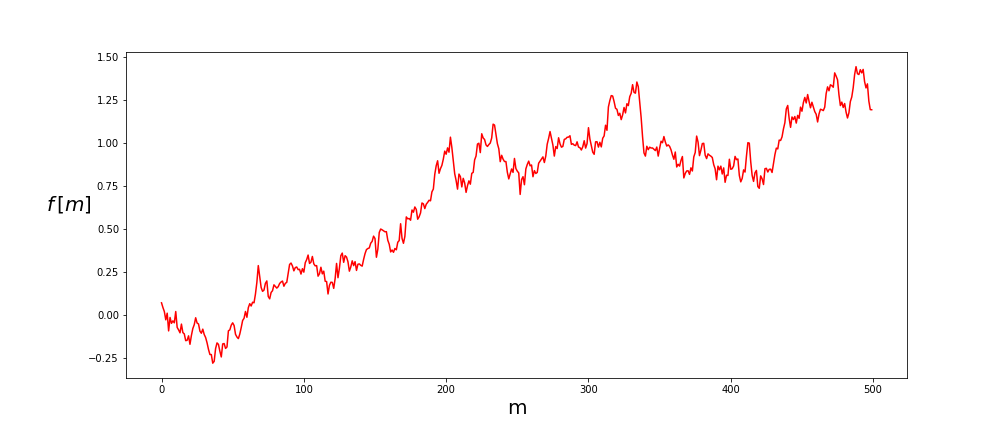
\includegraphics[width=0.95\textwidth]{figures/neural_networks/unsmoothed.png}
        \caption{Noisy function \(f\) (Wiener process sample).}\label{fig:convnoisy}
    \end{subfigure}

    \begin{subfigure}[b]{.49\textwidth}
        \centering
        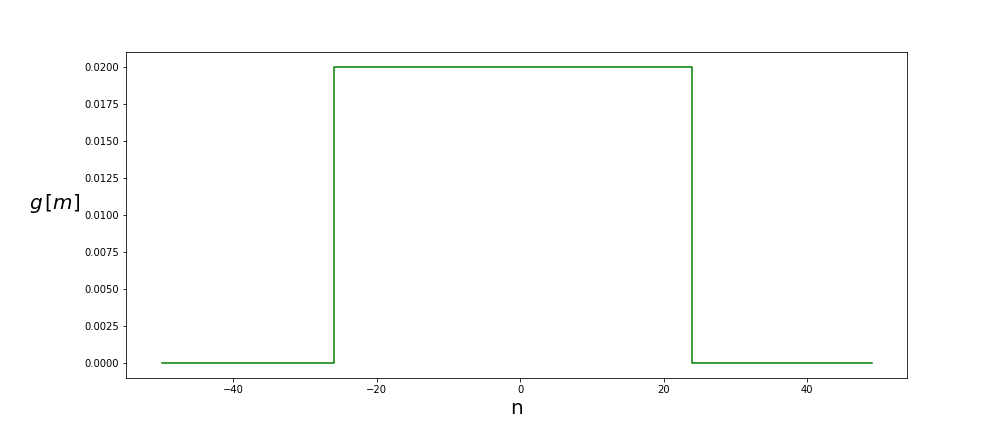
\includegraphics[width=0.95\textwidth]{figures/neural_networks/kernel.png}
        \caption{Heaviside function (low-pass filter \(g\)).}\label{fig:convfilter}
    \end{subfigure}
    \begin{subfigure}[b]{.49\textwidth}
        \centering
        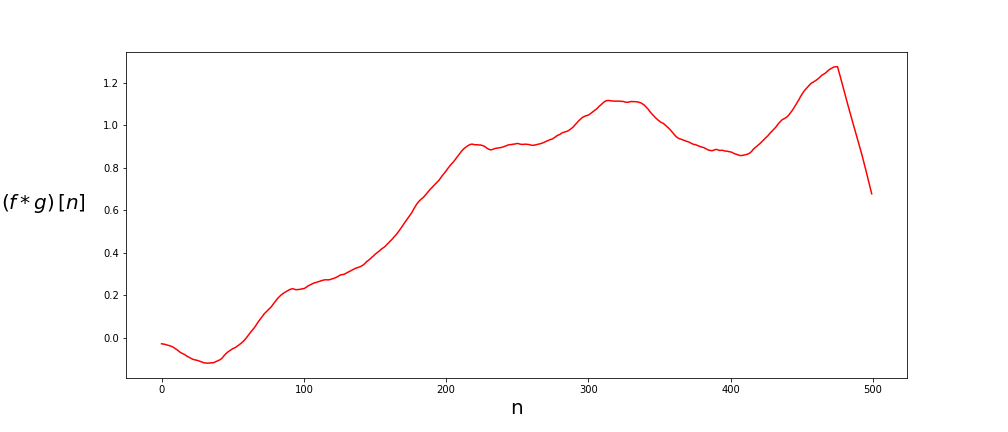
\includegraphics[width=0.95\textwidth]{figures/neural_networks/smoothed.png}
        \caption{Smoothed (low-pass filtered) \(f * g\).}\label{fig:convsmooth}
    \end{subfigure}
    \caption{Convolution as filtering.}\label{fig:convfiltering}
\end{figure}